\documentclass[twocolumn,a4j]{jsarticle}
\setlength{\topmargin}{-20.4cm}
\setlength{\oddsidemargin}{-10.4mm}
\setlength{\evensidemargin}{-10.4mm}
\setlength{\textwidth}{18cm}
\setlength{\textheight}{26cm}

\usepackage[top=15truemm,bottom=20truemm,left=20truemm,right=20truemm]{geometry}
\usepackage[latin1]{inputenc}
\usepackage{amsmath}
\usepackage{amsfonts}
\usepackage{amssymb}
\usepackage[dvipdfmx]{graphicx}
\usepackage[hang,small,bf]{caption}
\usepackage[subrefformat=parens]{subcaption}
\usepackage[dvipdfmx]{color}
\usepackage{listings}
\usepackage{listings,jvlisting}
\usepackage{geometry}
\usepackage{framed}
\usepackage{color}
\usepackage[dvipdfmx]{hyperref}
\usepackage{ascmac}
\usepackage{enumerate}
\usepackage{tabularx}
\usepackage{cancel}
\usepackage{scalefnt}
\usepackage{overcite}
\usepackage{otf}
\usepackage{multicol}

\renewcommand{\figurename}{Fig.}
\renewcommand{\tablename}{Table }

\lstset{
basicstyle={\ttfamily},
identifierstyle={\small},
commentstyle={\smallitshape},
keywordstyle={\small\bfseries},
ndkeywordstyle={\small},
stringstyle={\small\ttfamily},
frame={tb},
breaklines=true,
columns=[l]{fullflexible},
xrightmargin=0zw,
xleftmargin=3zw,
numberstyle={\scriptsize},
stepnumber=1,
numbersep=1zw,
lineskip=-0.5ex
}

% キャプション後ろのダブルコロンを消す
\makeatletter
\long\def\@makecaption#1#2{%
  \vskip\abovecaptionskip
  \iftdir\sbox\@tempboxa{#1\hskip1zw#2}%
    \else\sbox\@tempboxa{#1 #2}%
  \fi
  \ifdim \wd\@tempboxa >\hsize
    \iftdir #1\hskip1zw#2\relax\par
      \else #1 #2\relax\par\fi
  \else
    \global \@minipagefalse
    \hbox to\hsize{\hfil\box\@tempboxa\hfil}%
  \fi
  \vskip\belowcaptionskip}
\makeatother

% タイトル
\makeatletter
\def\@maketitle
{
\begin{center}
{\LARGE \@title \par}
\end{center}
\begin{flushright}
{\large \@date 報告書 No.24}\\
{\large M1 \@author}
\end{flushright}
\par\vskip 1.5em
}
\makeatother

\author{来代 勝胤}
\title{令和4年度 4月 第1週 報告書}
\date{2022/4/11}

\begin{document}
\columnseprule=0.1mm
\maketitle

\section*{シミュレーションの内容について}

\section*{Die drehstr\"{o}mung \"{u}ber festem grunde}

\section{地面近くにおける回転}

回転円盤近傍の流体を考える.
静止する板があり,遠く離れた距離に一定の速度で回転する円盤がある.
重要な影響の1つは,円盤近くの流体が遠心力によって
外側へ投げ出される.放射状に投げ出された流体は
軸方向に流れる流体によって置換される.
静止している壁付近の粒子の周速は減少し,
半径方向の遠心力は大幅に減少する.
一方で,半径方向の圧力勾配は変わらないため
静止壁付近の粒子が内側に流れることによって補完される.

\begin{figure}[htbp]
  \footnotesize
  \begin{center}
    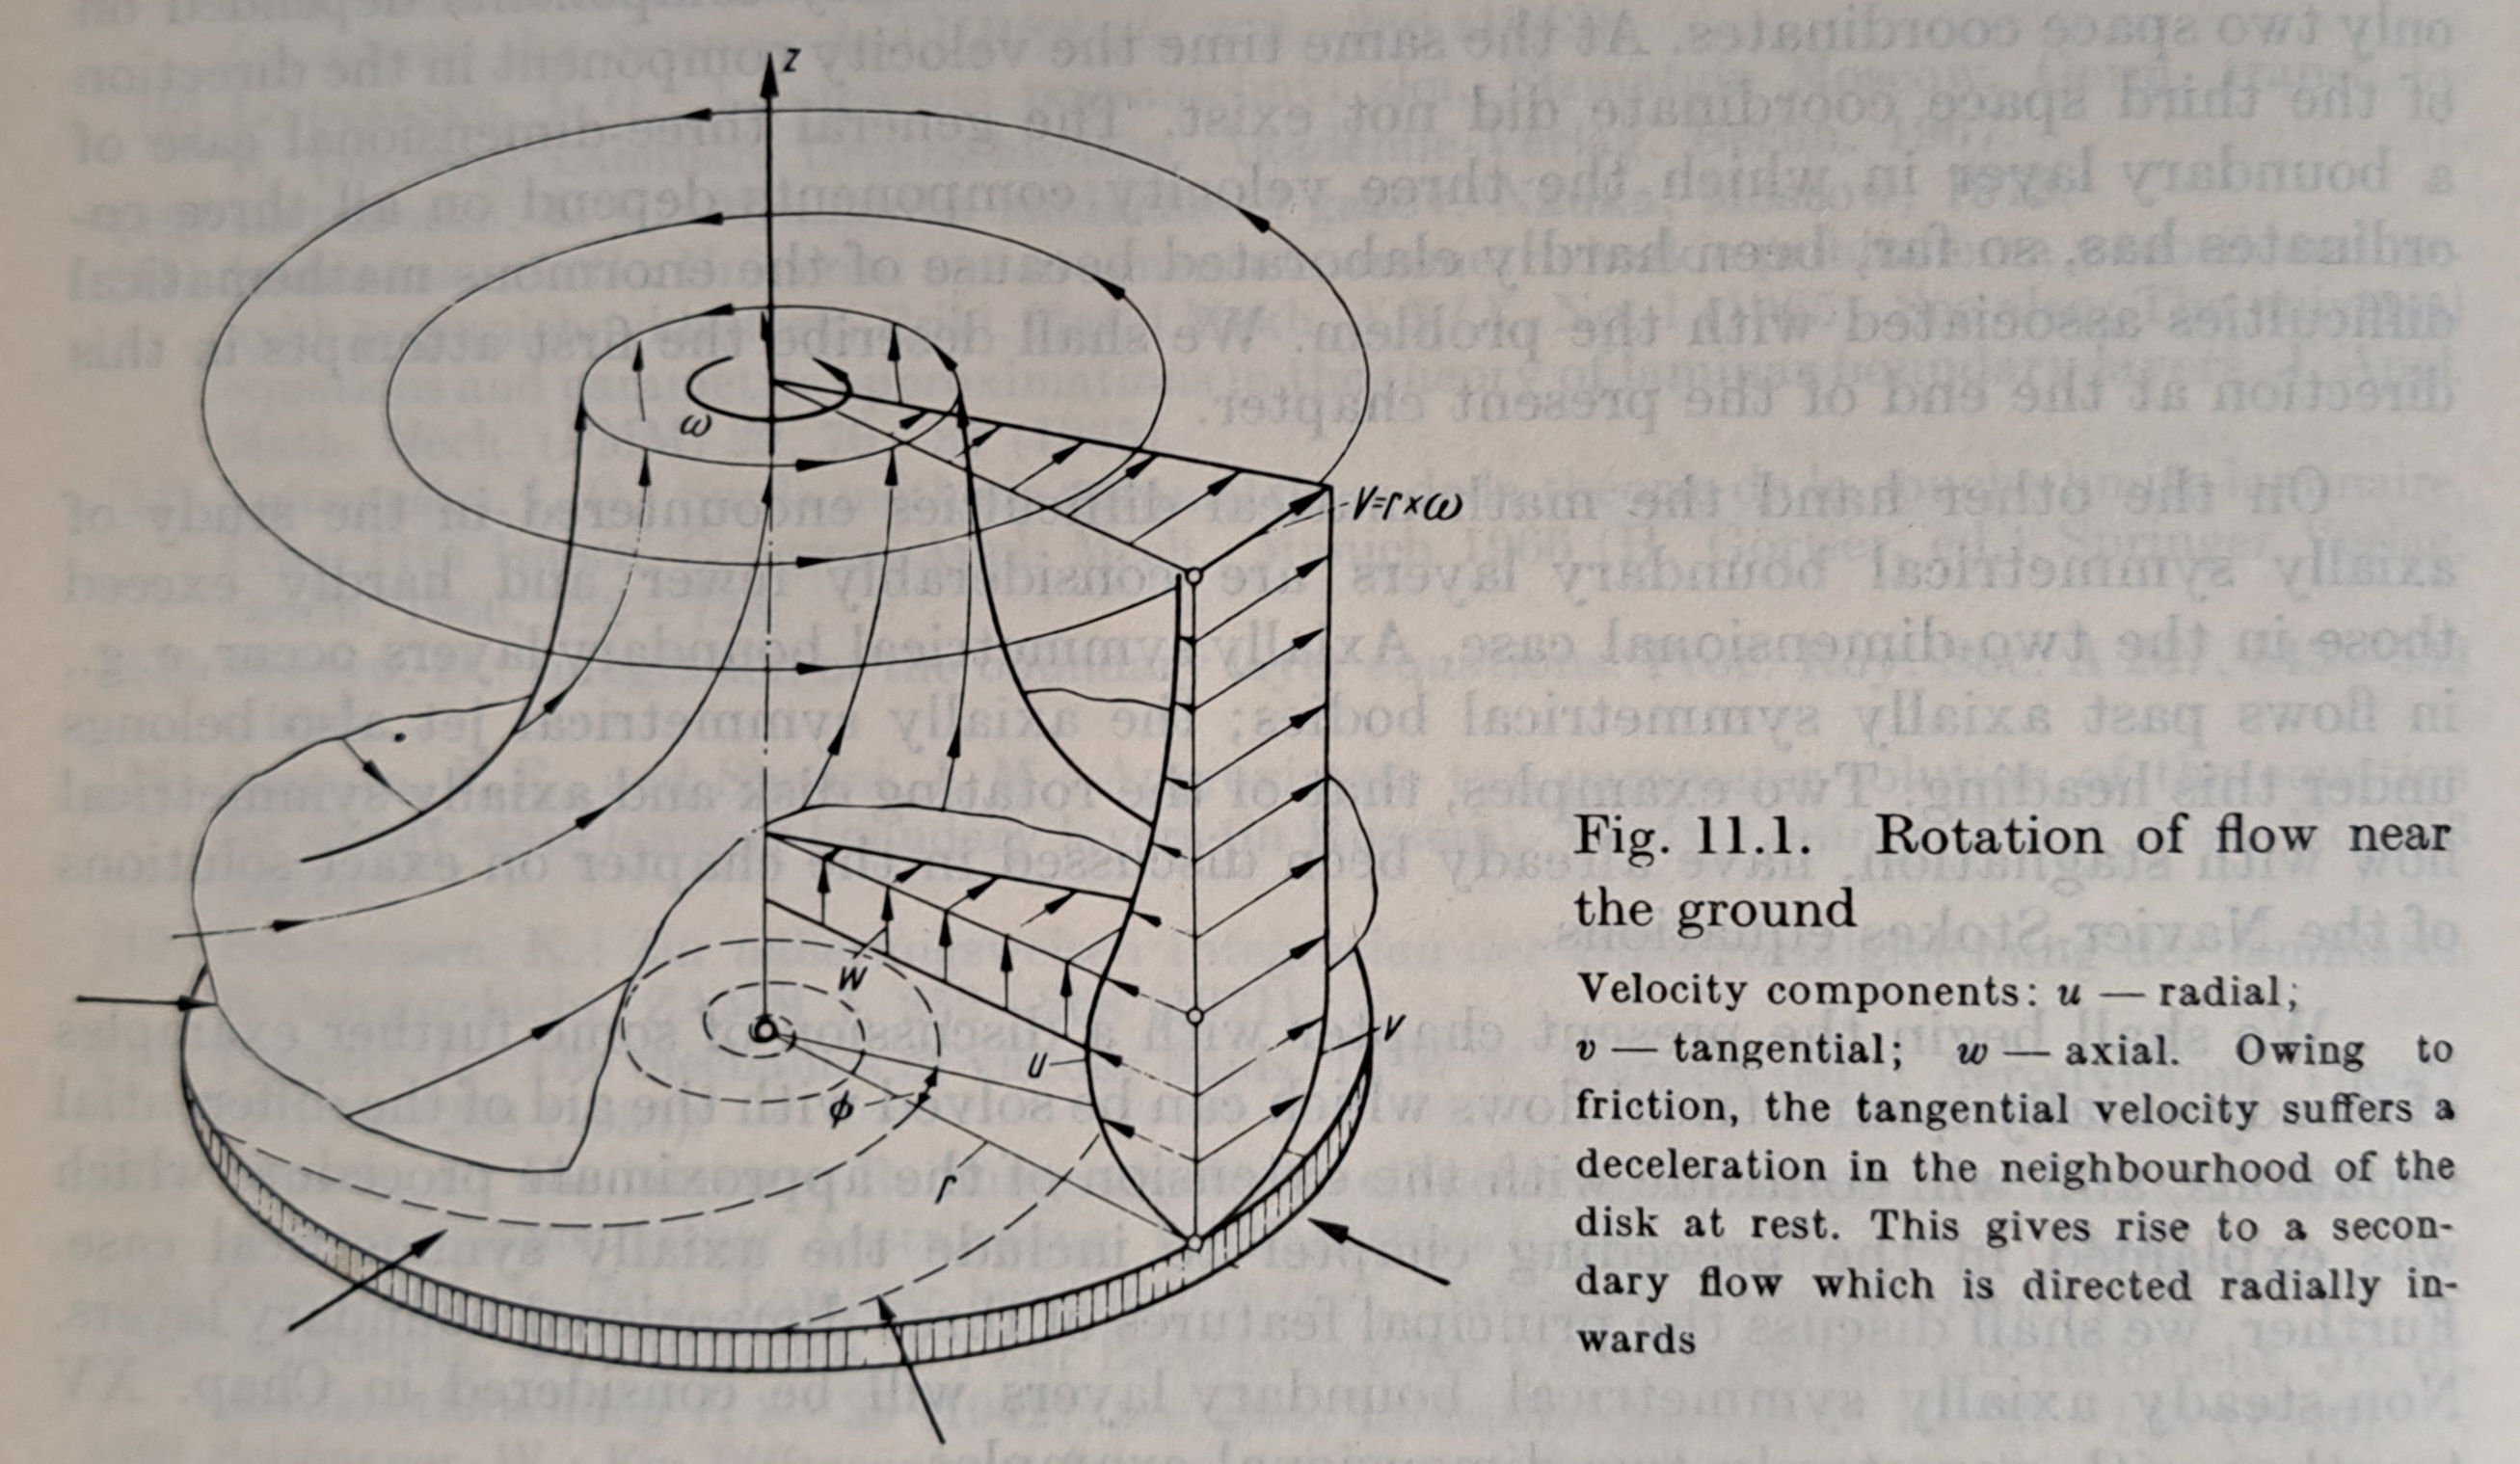
\includegraphics[width=80mm]{../images/Boundary-Layer_Theory_Fig.11.1.jpg}
    \caption{Rotation of flow near the ground ([1] P.226)}
  \end{center}
\end{figure}

\section{数学的モデル}

\begin{table}[hbtp]
  \label{table:data_type}
  \caption{モデルの条件}
  \centering
  \begin{tabular}{ c | c }
    \hline
    円柱極座標系     & $r, \phi, z$ \\ \hline
    静止壁の位置     & $z = 0$      \\ \hline
    回転壁の回転速度 & $\omega$     \\ \hline
    半径方向速度     & $u$          \\ \hline
    周方向速度       & $v$          \\ \hline
    軸方向速度       & $w$          \\ \hline
  \end{tabular}

  \begin{itemize}
    \item [※] $\phi$ は$z$軸に対称な流れであると仮定しているため,
          ナビエストークス方程式において考慮しない可能生がある.
  \end{itemize}
\end{table}

\section{数値解法}

\subsection*{支配方程式}

$\blacksquare$ \textgt{ナビエ・ストークス方程式}
\begin{eqnarray*}
  u \frac{\partial u}{\partial r} + w \frac{\partial u}{\partial z} - \frac{v^2}{r} &=& -\frac{1}{\rho}\frac{\partial p}{\partial r} + \nu \left\{\frac{\partial^2 u}{\partial r^2} + \frac{\partial}{\partial r}\left(\frac{u}{r}\right) + \frac{\partial^2 u}{\partial z^2}\right\}\\
  u \frac{\partial v}{\partial r} + w \frac{\partial v}{\partial z} + \frac{uv}{r} &=& \nu \left\{\frac{\partial^2 v}{\partial r^2} + \frac{\partial}{\partial r}\left(\frac{v}{r}\right) + \frac{\partial^2 v}{\partial z^2}\right\}\\
  u \frac{\partial w}{\partial r} + w \frac{\partial w}{\partial z} &=& -\frac{1}{\rho}\frac{\partial p}{\partial z} + \nu \left\{\frac{\partial^2 w}{\partial r^2} + \frac{1}{r}\frac{\partial w}{\partial r} + \frac{\partial^2 w}{\partial z^2}\right\}\\
\end{eqnarray*}


$\blacksquare$ \textgt{連続の式}
\begin{eqnarray*}
  \frac{1}{r} \frac{\partial \left(ur\right)}{\partial r} + \frac{\partial w}{\partial z} &=& 0\\
\end{eqnarray*}

\subsection*{境界条件}
\begin{table}[hbtp]
  \centering
  \begin{tabular}{ c c c c }
    $z=0$      & $u=0$ & $v=0$        & $w=0$ \\
    $z=\infty$ & $u=0$ & $v=r \omega$ &       \\
  \end{tabular}
\end{table}

\subsection*{無次元座標}
\begin{eqnarray*}
  \zeta = z \sqrt{\frac{\omega}{\nu}}
\end{eqnarray*}

\begin{eqnarray*}
  u &=& r \omega F \left(\zeta\right)\\
  v &=& r \omega G \left(\zeta\right)\\
  w &=& \sqrt{r \omega} H \left(\zeta\right)
\end{eqnarray*}

\begin{eqnarray*}
  \frac{1}{\rho} \frac{\partial p}{\partial r} = r \omega ^2
\end{eqnarray*}

\begin{figure}[htbp]
  \footnotesize
  \begin{center}
    \includegraphics[width=80mm]{../images/function.jpg}
    \caption{Rotation of flow near the ground ([1] P.226)}
  \end{center}
\end{figure}

\begin{table}[hbtp]
  \centering
  \begin{tabular}{| r | r | r | r |}
    \hline
    $\zeta$  & $F$     & $G$    & $H$    \\ \hline \hline
    0.0      & 0.000   & 0.000  & 0.000  \\ \hline
    0.5      & -0.3487 & 0.3834 & 0.1944 \\ \hline
    1.0      & -0.4788 & 0.7354 & 0.6241 \\ \hline
    1.5      & -0.4496 & 1.0134 & 1.0987 \\ \hline
    2.0      & -0.3287 & 1.1924 & 1.4929 \\ \hline
    2.5      & -0.1762 & 1.2721 & 1.7459 \\ \hline
    3.0      & -0.0361 & 1.2714 & 1.8496 \\ \hline
    3.5      & 0.0663  & 1.2182 & 1.8308 \\ \hline
    4.0      & 0.1227  & 1.1413 & 1.7325 \\ \hline
    4.5      & 0.1371  & 1.064  & 1.5995 \\ \hline
    5.0      & 0.1210  & 1.0016 & 1.4685 \\ \hline
    5.5      & 0.0878  & 0.9611 & 1.3632 \\ \hline
    6.0      & 0.0499  & 0.9427 & 1.2944 \\ \hline
    6.5      & 0.0162  & 0.9407 & 1.2620 \\ \hline
    7.0      & -0.0084 & 0.9530 & 1.2585 \\ \hline
    7.5      & -0.0223 & 0.9693 & 1.2751 \\ \hline
    8.0      & -0.0268 & 0.9857 & 1.3004 \\ \hline
    8.5      & -0.0234 & 0.9991 & 1.3264 \\ \hline
    9.0      & -0.0179 & 1.0078 & 1.3477 \\ \hline
    9.5      & -0.0102 & 1.0119 & 1.3617 \\ \hline
    10.0     & -0.0033 & 1.0121 & 1.3683 \\ \hline
    10.5     & 0.0018  & 1.0099 & 1.3689 \\ \hline
    11.0     & 0.0047  & 1.0065 & 1.3654 \\ \hline
    11.5     & 0.0057  & 1.0031 & 1.3601 \\ \hline
    12.0     & 0.0052  & 1.0003 & 1.3546 \\ \hline
    12.5     & 0.0038  & 0.9984 & 1.3500 \\ \hline
    $\infty$ & 0.0000  & 1.0000 & 1.3494 \\ \hline
  \end{tabular}
\end{table}

\end{document}